% Project proposal (Steps 1-2 only). Build: latexmk -pdf proposal.tex
% Speaker notes: build proposal-notes.tex (same content, notes shown on a second page).
\documentclass[aspectratio=169,11pt]{beamer}
\usetheme[progressbar=frametitle,numbering=fraction]{metropolis}
\usepackage{booktabs}
\usepackage{graphicx}
\usepackage{tabularx}
\usepackage{array}
\graphicspath{{../outputs/figures/}}
% Auto-generated by src/data/eda.py -- do not edit by hand.
\newcommand{\nRddAnnotated}{35{,}984}
\newcommand{\nRddPositive}{3{,}610}
\newcommand{\pctRddPositive}{10}
\newcommand{\nRddBoxes}{6{,}458}
\newcommand{\pctRddTopTwo}{81}
\newcommand{\nRddTrain}{3{,}160}
\newcommand{\nRddVal}{638}
\newcommand{\nA}{708}
\newcommand{\nB}{708}
\newcommand{\nC}{681}
\newcommand{\nD}{676}
\newcommand{\nMwpd}{1{,}357}
\newcommand{\nMwpdRainyTrain}{340}
\newcommand{\nDHalf}{336}
\newcommand{\nBoxA}{1{,}046}
\newcommand{\nBoxC}{1{,}450}
\newcommand{\nBoxD}{2{,}658}
\newcommand{\pctSmallRdd}{26}
\newcommand{\pctSmallMwpd}{1}
\newcommand{\blockSize}{50}
\newcommand{\negRatioPct}{20}


\providecommand{\shownotes}{0}
\ifnum\shownotes=1
  \setbeameroption{show notes on second screen=right}
\fi

\newcommand{\researchq}[2]{\textbf{RQ#1.}~#2}

\title{Rain-Robust Pothole Detection}
\subtitle{How much does rain hurt a pothole detector, and what helps?\\[2pt]
  \small CSE36501 Deep Learning --- Project Proposal}
\author{[Name] \quad ([Student ID])}
\institute{UNIST, Fall 2026}
\date{November 6, 2026}

\begin{document}

% ---------------------------------------------------------------- 1
\maketitle
\note{%
Hello, I am [Name]. My project is about rain-robust pothole detection.
In short, I want to measure how much a pothole detector that was trained on clear-weather
images breaks down when it rains, and then test which fix helps the most.
In this proposal I will cover the problem definition and the datasets; models and
experiments will come in the final presentation.}

% ---------------------------------------------------------------- 2
\begin{frame}{Motivation}
  \begin{itemize}
    \item Potholes cause accidents, tyre and suspension damage, and costly repairs.
    \item Vision-based road monitoring and driver assistance increasingly detect them
          automatically from vehicle cameras.
    \item \alert{Rain is exactly when potholes are most dangerous} --- and hardest to see:
      \begin{itemize}
        \item water fills the hole and hides its depth and edges,
        \item wet asphalt reflects light; rain streaks and darkness lower contrast.
      \end{itemize}
    \item Public pothole detectors are trained almost entirely on \emph{clear-weather} images.
  \end{itemize}
  \vfill
  \centering\large A detector that fails in the rain fails when it is needed most.
\end{frame}
\note{%
Potholes are not just an annoyance: they damage vehicles and cause accidents, and many
cities and car makers now try to detect them automatically from cameras.
The problem is that rain is precisely the condition where potholes are most dangerous,
because water fills them and hides their depth, and wet asphalt reflects light.
At the same time, almost all public training data is captured in good weather.
So there is a mismatch between where these models are trained and where they matter most.}

% ---------------------------------------------------------------- 3
\begin{frame}{Problem statement}
  \textbf{Task.} Single-class object detection (bounding boxes) of potholes in
  vehicle- or pedestrian-view road images.

  \medskip
  \textbf{Setting.} Train on clear-weather road images; test on clear, synthetic-rain
  and real-rain images.

  \bigskip
  \begin{itemize}
    \item[] \researchq{1}{How much does a pothole detector trained only on clear-weather images
      degrade under rain?}
    \item[] \researchq{2}{Can synthetic rain overlays serve as a proxy for real rainy conditions?}
    \item[] \researchq{3}{Which strategy improves rain robustness most: (a) synthetic-rain
      augmentation, (b) architectural change (attention module), or (c) test-time
      deraining?}
  \end{itemize}
\end{frame}
\note{%
Formally, the task is single-class pothole detection with bounding boxes.
I train on clear-weather images and test under three conditions: clear, synthetic rain,
and real rain. This gives three research questions.
First, how large is the drop under rain?
Second, does synthetic rain behave like real rain, so that we could benchmark and train
with cheap synthetic data?
And third, among three common fixes, augmentation, an attention module, and a deraining
pre-processor, which one actually helps most?}

% ---------------------------------------------------------------- 4
\begin{frame}{Datasets}
  \footnotesize
  \renewcommand{\arraystretch}{0.95}
  \begin{tabularx}{\textwidth}{@{}>{\bfseries}l X X@{}}
    \toprule
    & RDD2022 \normalfont(Arya et al., 2024) & MWPD \normalfont(Parvin et al., 2025) \\
    \midrule
    Role & clear-weather train / val / test & external test: real normal vs.\ rain \\
    Source & vehicle-mounted cameras \& phones, 6 countries & mixed web, news and
      phone images \\
    Size & 47{,}420 images, 4 damage types; we keep \textbf{D40 = pothole}
      (\nRddPositive{} positive images, \nRddBoxes{} boxes) & \nMwpd{} images, 640$\times$640 \\
    Labels, license & Pascal VOC XML; CC BY 4.0 & YOLO txt, 1 class; CC BY 4.0 \\
    Conditions & clear daylight & normal / rainy; day / twilight / night \\
    \bottomrule
  \end{tabularx}

  \smallskip
  \begin{itemize}\scriptsize
    \setlength{\itemsep}{1pt}
    \item \textbf{Why these:} RDD2022 is the largest public multi-country road-damage set;
      MWPD is, to our knowledge, the only public pothole set with real rain.
    \item China\_Drone excluded (top-down drone view $\neq$ vehicle view).
    \item MWPD ships \alert{without weather labels} $\Rightarrow$ every image was tagged
      normal/rainy (pre-tag + manual review).
  \end{itemize}
\end{frame}
\note{%
I use two datasets. RDD2022 is the large multi-country road damage dataset from the CRDDC
challenge, with about forty-seven thousand images. It has several damage classes; I keep
only D40, which is the pothole class. I drop the China drone subset because it is shot from
above and does not match a car's view.
For real rain I use MWPD, the Multi-Weather Pothole Detection dataset, which contains
normal and rainy images. One important finding: although MWPD describes rainy conditions,
the files carry no weather label, so I tagged every image as normal or rainy myself.}

% ---------------------------------------------------------------- 5
\begin{frame}{Dataset analysis}
  \begin{columns}[T]
    \begin{column}{0.5\textwidth}
      \centering
      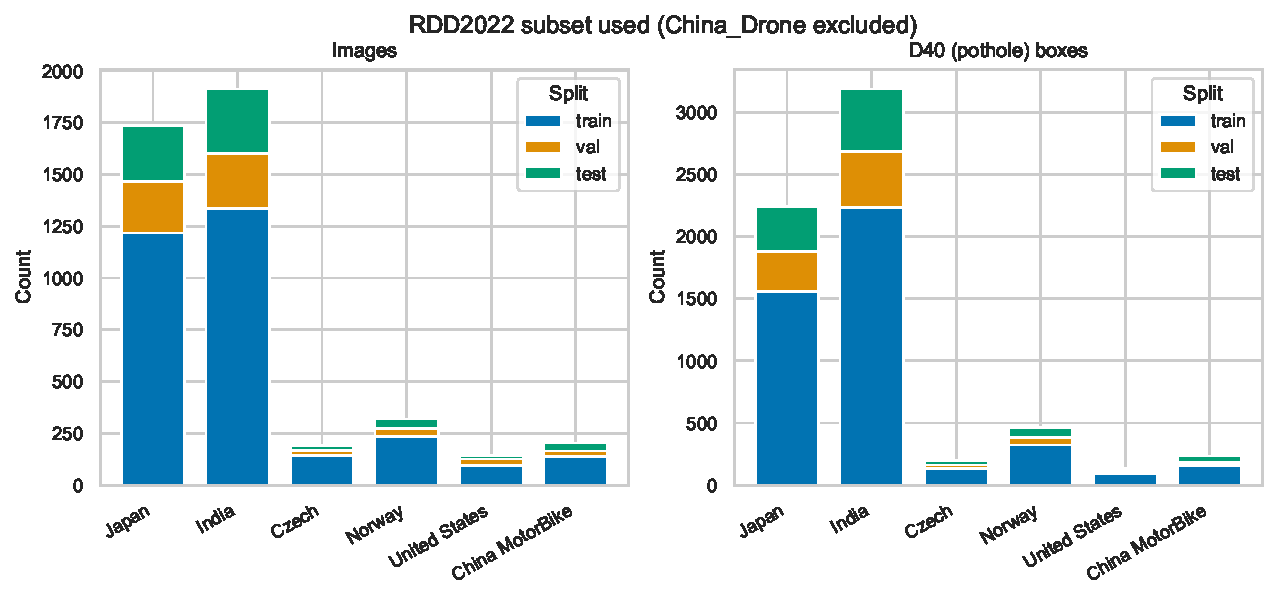
\includegraphics[width=\linewidth]{fig_rdd_country_counts}
      \footnotesize Only \pctRddPositive\% of annotated RDD images contain a pothole;
      Japan + India hold \pctRddTopTwo\% of them.
    \end{column}
    \begin{column}{0.5\textwidth}
      \centering
      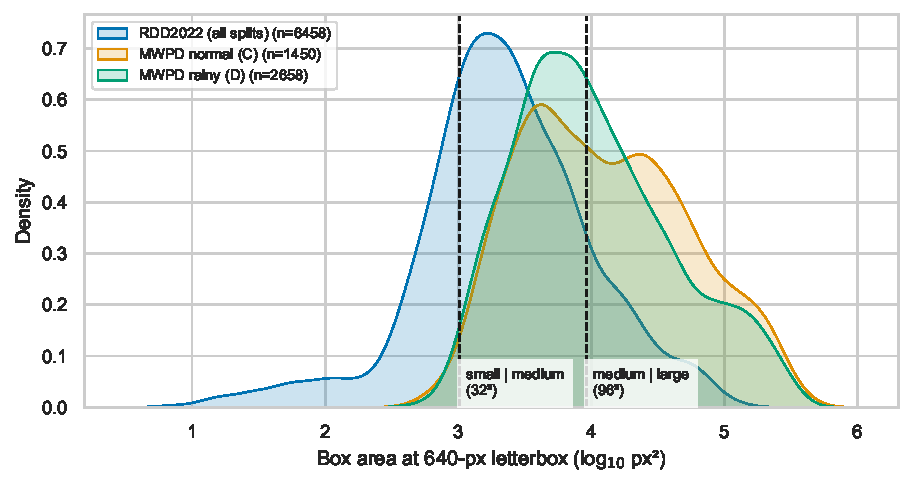
\includegraphics[width=\linewidth]{fig_box_size}
      \footnotesize MWPD potholes are much larger (close-up photos):
      \pctSmallRdd\% of RDD boxes are COCO-small vs.\ \pctSmallMwpd\% in MWPD.
    \end{column}
  \end{columns}
  \medskip
  \footnotesize\textbf{Leakage-safe split:} RDD frames are grouped into blocks of
  \blockSize{} consecutive frames per country; whole blocks go to train/val/test (70/15/15).
  Negatives capped at \negRatioPct\% per split.
\end{frame}
\note{%
Two things stand out in the data. On the left: potholes are rare in RDD; only about one
in ten annotated images contains one, and most come from Japan and India.
On the right: object size differs a lot. RDD potholes are small and far away, as seen from
a dashcam, while MWPD potholes are mostly large close-ups. So part of any drop from RDD
to MWPD will be a size and viewpoint effect, not weather, and I will report size-wise AP
to separate them.
Finally, because RDD contains video-like consecutive frames, I split by blocks of fifty
frames so near-identical images never end up in both train and test.}

% ---------------------------------------------------------------- 6
\begin{frame}{Test-set design}
  \centering\footnotesize
  \begin{tabular}{@{}llrl@{}}
    \toprule
    ID & Composition & Images & Purpose \\
    \midrule
    A & RDD2022 own test split (clear) & \nA & baseline \\
    B1/B2/B3 & \emph{same images} as A + synthetic drizzle / heavy / torrential & \nB{} each
      & pure rain effect \\
    C & MWPD normal weather & \nC & domain gap \\
    D & MWPD rainy & \nD & real rain effect \\
    \bottomrule
  \end{tabular}

  \smallskip
  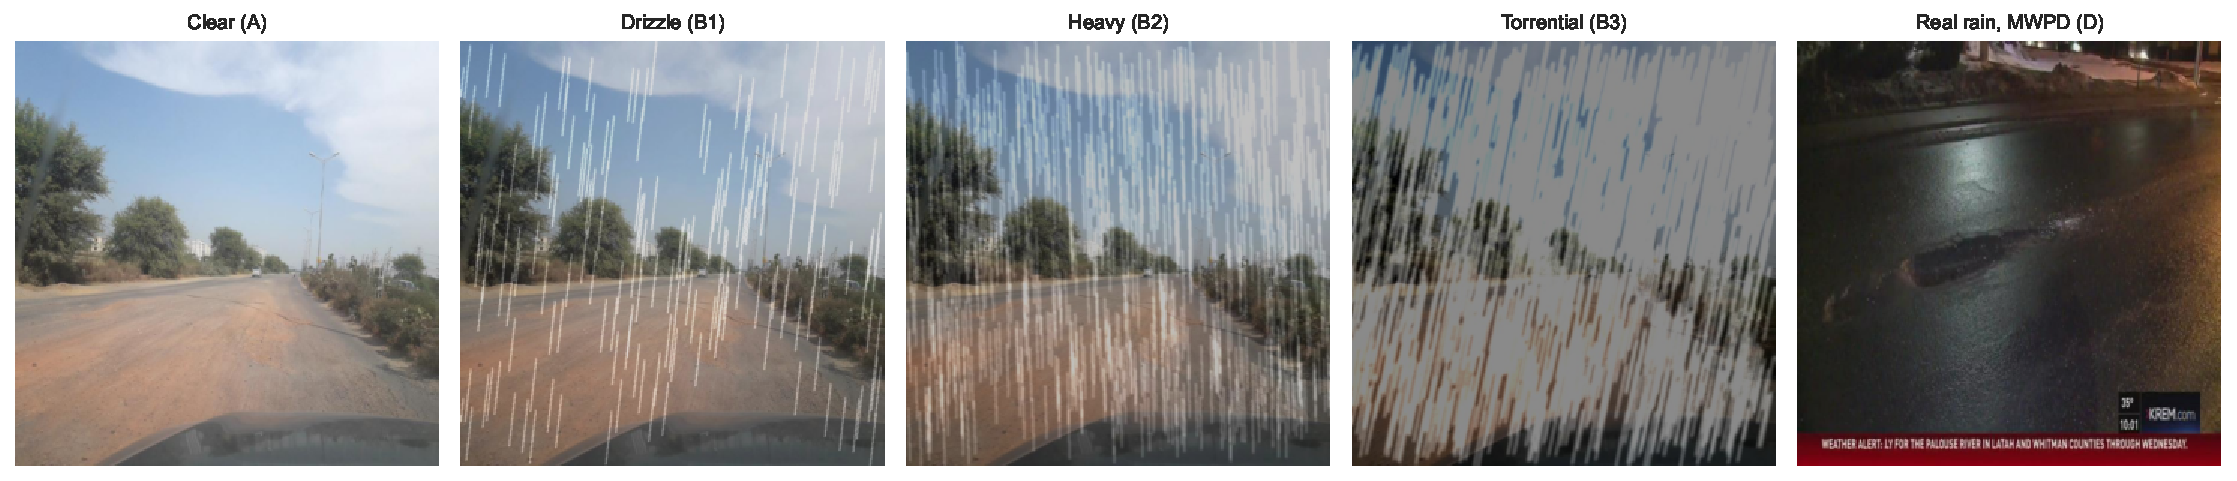
\includegraphics[width=0.88\textwidth]{fig_rain_levels}

  \footnotesize
  A$\to$B: synthetic rain only \quad
  A$\to$C: domain (country, camera, size) \quad
  C$\to$D: real rain, same source \quad
  \alert{(A$\to$B) vs.\ (C$\to$D): is synthetic rain a valid proxy? (RQ2)}
\end{frame}
\note{%
This is the core of the design. Set A is my clean RDD test split. B1 to B3 are the very same
images with synthetic rain of increasing strength, so any change from A to B is caused by
rain alone. C and D come from MWPD: normal and rainy. A to C measures the domain gap, and
C to D measures the effect of real rain within the same source.
Comparing the A-to-B drop with the C-to-D drop answers whether synthetic rain is a fair
stand-in for real rain. Note that synthetic rain only adds streaks, darkening and blur; it
cannot reproduce water-filled potholes or reflections, which is exactly what we may see in D.}

% ---------------------------------------------------------------- 7
\begin{frame}{Plan \& timeline}
  \small
  \begin{tabularx}{\textwidth}{@{}l X l@{}}
    \toprule
    Step & Content & Status \\
    \midrule
    1--2 & Problem, datasets, splits, test sets A--D & \alert{done (this talk)} \\
    3 & Models: YOLOv8n/s, RT-DETR-L, YOLOv8s + CBAM (ours);
        strategies: clean, rain-aug, deraining, real-rain upper bound & next \\
    4 & Evaluation: mAP50(-95), recall, relative drop, size-wise AP, FPS; 3 seeds & \\
    5 & Analysis, failure cases, Grad-CAM; report \& final video & \\
    \bottomrule
  \end{tabularx}

  \bigskip
  \footnotesize Compute: one RTX 3090 (24\,GB). Everything is scripted
  (\texttt{make data}, \texttt{make train}, \dots) and seeded for reproducibility.
\end{frame}
\note{%
Steps one and two, the problem and the data, are finished and are what I presented today.
Next I will train four detectors, two YOLOv8 sizes, the transformer-based RT-DETR, and my own
YOLOv8 variant with CBAM attention, under clean training, synthetic-rain augmentation,
test-time deraining, and real-rain training as an upper bound. I will evaluate them on all
six test sets with three seeds each, and finish with failure analysis and Grad-CAM.
Thank you.}

\end{document}
